\documentclass[a4paper,11pt]{article}
\usepackage[a4paper,hmargin=2.5cm,vmargin=2.5cm]{geometry}
\usepackage{amsmath}
\usepackage{amssymb}
\usepackage{gensymb}
\usepackage{bm}
\usepackage{rotating}
\usepackage{booktabs}
\usepackage{mathtools}
\usepackage{bm}
\usepackage{esvect}
\usepackage[english]{babel}
\usepackage{hyperref}
\usepackage{graphicx}
\usepackage{array}
\usepackage{url}
\usepackage{siunitx}
\usepackage{cite}
\usepackage{pstricks}
\usepackage{chemformula}
\usepackage{mathtools}
\usepackage{chngcntr}
\graphicspath{{figures/}}
\usepackage[toc]{glossaries-extra}
\usepackage{listings}
\usepackage{listing}

\counterwithin{figure}{section}
\DeclarePairedDelimiter\abs{\lvert}{\rvert}
\DeclarePairedDelimiter\norm{\lVert}{\rVert}
\makeatletter
\newsavebox\myboxA
\newsavebox\myboxB
\newlength\mylenA

\newcommand*\xoverline[2][0.75]{%
    \sbox{\myboxA}{$\m@th#2$}%
    \setbox\myboxB\null% Phantom box
    \ht\myboxB=\ht\myboxA%
    \dp\myboxB=\dp\myboxA%
    \wd\myboxB=#1\wd\myboxA% Scale phantom
    \sbox\myboxB{$\m@th\overline{\copy\myboxB}$}%  Overlined phantom
    \setlength\mylenA{\the\wd\myboxA}%   calc width diff
    \addtolength\mylenA{-\the\wd\myboxB}%
    \ifdim\wd\myboxB<\wd\myboxA%
       \rlap{\hskip 0.5\mylenA\usebox\myboxB}{\usebox\myboxA}%
    \else
        \hskip -0.5\mylenA\rlap{\usebox\myboxA}{\hskip 0.5\mylenA\usebox\myboxB}%
    \fi}
\makeatother

\newcommand{\mysection}[2]{\setcounter{section}{#1}\addtocounter{section}{-1}\section{#2}}
\makeglossaries

\newglossaryentry{pi}
{
	name={Raspberry Pi Zero},
	description={or Pi, or Pi Zero, is a $\SI{1}{\giga\hertz}$ single-core computer with a $\SI{512}{\mega\byte}$.}
}

\newglossaryentry{tdoa}
{
	name={time difference of arrival},
	description={or TDoA, is a technique used in signal processing and localisation for computing the position of a of a sound source by measuring the difference in the time of arrival of a signal at multiple sensors or receivers.}
}

\newglossaryentry{toa}
{
	name={time of arrival},
	description={or ToA, refers to the time $t_i$ when an acoustive wave arrives at a microphone $m_i$.}
}

\newglossaryentry{aoa}
{
	name={angle of arrival},
	description={or AoA, refers to the angle between the horizontal axis of microphone pairs and the direction from which an acoustic wave arrives at a given microphone. }
}

\newglossaryentry{gcc}
{
	name={generalized cross correlation with phase transform},
	description={is an algorithm used in signal processing to estimate the time delay or time difference of arrival between two signals received by separate sensors or microphones.}
}

\newglossaryentry{source}
{
	name={source},
	description={an object located in a 3D space which emits an acoustic wave.}
}

\newglossaryentry{msigs}
{
	name={microphone signal},
	description={refers to the audio signal detected by a microphone audio sensor.}
}
\renewcommand*\contentsname{Table of Contents}
\begin{document}

\pagenumbering{gobble}

\begin{titlepage}
	
	\thispagestyle{empty}
	\centering 
	{\Large\bfseries University of Cape Town}
	
	\begin{figure}[ht!]
		\centering
		{
\includegraphics[scale=0.25]{UCT_Logo.jpg}}
		\label{Schematic:1}
	\end{figure}
	
	\vspace{0.809cm}
	
	{\Large\bfseries EEE3097S}
	
	\vspace{0.809cm}
	
	{\Large\bfseries Engineering Design: Electrical \& Computer Engineering}
	
	\vspace{4.472cm}
	
	{\LARGE\bfseries First Progress Report\\Cover Page}
	
	\vspace{1.00cm}
	
	
	\vspace{5.008cm}
	
	{\large\bfseries ~Group: 9\\ NJMLUN002 || NKMMOR001 || PRTCHA018}
	
	\vspace{0.809cm}
	
	{\bfseries 18 September 2023\\}
	
	\vspace{4.80cm}
	
	{\LARGE\bfseries Simulating Acoustic Triangulation Using} 
	
	\vspace{0.189cm}
	
	{\LARGE\bfseries Time Difference of Arrival Measurements}
	
	\vspace{0.189cm}
	
	{\Large\bfseries Prepared for:\\}
	
	\vspace{0.809cm}
	{\text  Faculty of Engineering and Built Environment\\}
	
	\vspace{0.189cm}
	
	{\text Department of Electrical Engineering\\}
	
	\vspace{0.189cm}
	
	{\text University of Cape Town}
	
	\vspace{3.30cm}
	
	{\Large\bfseries Prepared by:\\}
	\vspace{0.809cm}
	{\text Group 9}
	
	\vspace{3.30cm}
	
	{\Large\bfseries Date:\\}
	\vspace{0.809cm}
	{\text 18/09/2021} 
	
	\vspace{3.30cm}
	
	{\Large\bfseries Keywords:\\}
	\vspace{0.809cm}
	{\text Acoustic triangulation, time difference of arrival, sound source tracking, generalized cross-correlation}
	
\end{titlepage}
\newpage

\pagenumbering{roman}

\addcontentsline{toc}{section}{Terms of Reference}

\section*{Terms of Reference}
This report was requested by the Electrical Engineering Department at the University of Cape Town, for the Engineering Design 3rd year course, on the 14th August 2023. This Terms of Reference outlines the scope and objectives for the preparation and submission of a comprehensive report on a simulation conducted to achieve sound source localization utilizing an array of microphones. This report is intended for engineering professionals and stakeholders.
\\\\
In particular, the department requires:

\begin{enumerate}
	\item A description of the simulation environment and tools used and explanation for chosen approach.
	\item  clear and separate sections for the subsystems to be simulated and the
	system as a whole, clearly describing the simulations and/or experiments run
	on the subsystems and the system as a whole.
	\item Present the overall system architecture, including the raspberry pi zeros and
	microphones.
	\item Describe how the distributed sensor network is structured, making sure to
	incorporate this structure in your simulation model.
	\item Explain the algorithms or techniques used for time difference of arrival
	(TDOA) calculation.
	\item Share the outcomes of the simulation experiments for the simulated
	subsystems and the system as a whole, clearly separating these results into
	their own individual sections.
	\item Present the accuracy and precision achieved in locating the acoustic signal
	within the grid.
	\item Recommend potential improvements or modifications to enhance the accuracy or efficiency of the system.
	\item Summary of the key findings from the simulation stage.
\end{enumerate}

\addcontentsline{toc}{section}{Summary}
\clearpage

\section*{Summary}
This report concerns the simulation of an acoustic triangulation system requested by the Electrical Engineering Department for locating the position of an object emitting an audio signal through air using four microphones as sensors and two Raspberry Pi Zero (Pi) single-board computers as the micro-control unit (MCU). 

\subsection*{Background and Motivation}
Acoustic triangulation plays a significant role in a variety of applications across a spectrum of domains. Acoustic triangulation can be applied in security systems, virtual reality, sound design and audio engineering, as well as medical technology. This report assimilates the principles and methodologies characterising acoustic triangulation through a description of the algorithms that were implemented in locating a sound source based on the location of an array of microphones. The department aims to use the results from the simulation in refining the practical hardware implementation. 

\subsection*{Objectives of Investigation and Methodology}
The purpose of this report is to describe the simulation setup and methodology, present and analyse simulation results, assess the accuracy and reliability of sound source localisation techniques, as well as provide recommendations for practical implementation and improvements.

\subsection*{Results of Investigation}

Time Delay Estimation Subsystem:\\\\
Our simulations demonstrated that the Time Delay Estimation Subsystem performs admirably in estimating time delays between microphone pairs. We utilized the GCC-PHAT algorithm to accurately compute these delays, even in the presence of mixed-frequency sound signals. The subsystem's performance was consistent, showcasing precise time delay estimations as the source's distance from the reference microphone increased. These results affirm the subsystem's robustness and effectiveness in capturing crucial time delay information.\\\\
Triangulation \& Sound-Tracking Subsystem:\\\\
The Triangulation \& Sound-Tracking Subsystem exhibited remarkable capabilities in localizing sound sources within a 3D space. Through Time Difference of Arrival (TDoA) measurements, we successfully determined the direction of arrival for sound sources. This method, which relies on angles adjacent to the longest sound paths between microphone pairs, consistently produced accurate sound source localization results. Moreover, our simulations highlighted the subsystem's potential for real-time sound source tracking, making it a valuable tool for applications requiring dynamic sound monitoring.
  
\subsection*{Conclusions}

Our investigation into acoustic triangulation for sound source localization and tracking has yielded promising results. The Time Delay Estimation Subsystem showcased its ability to provide precise time delay estimations, important for the accurate determination of sound source locations. The Triangulation \& Sound-Tracking Subsystem proved its effectiveness in localizing sound sources in a 3D space and tracking their movements with precision.

\subsection*{Recommendations}

Based on the facts that were collated and the conclusions that were drawn about the acoustic triangulation design, the following recommendations to improve the properties of the system have been made:

\begin{itemize}
	\item
	While our simulations provided valuable insights, it is recommended to conduct real-world testing to validate the system's performance under practical conditions. Consider implementing the system in controlled environments with actual sound sources to assess its accuracy and reliability.
	\item 
	Extend the investigation to evaluate the system's performance in the presence of background noise and multiple sound sources. Implement noise reduction techniques to enhance the system's robustness in complex acoustic environments.
	\item 
	Explore opportunities for optimizing the system's computational efficiency, particularly for real-time applications. This may involve hardware acceleration or algorithmic enhancements to reduce processing time
	\item 
	Investigate the feasibility of integrating the acoustic triangulation system into specific applications, such as security systems, virtual reality environments, and sound design tools. Assess the compatibility and potential for customization to meet specific user requirements.
	\item 
	Consider developing a user-friendly interface for configuring system parameters, visualizing sound source locations, and monitoring tracking results. User interface improvements can enhance the system's usability and accessibility.
	\item 
	Implement data logging and analysis features to record and analyze sound source localization results over time. This can be valuable for performance assessment and trend analysis.
	\item
	Develop calibration procedures to ensure accurate alignment of microphones and reference points. Calibration is essential for maintaining the system's accuracy over extended periods.
\end{itemize}
\printglossaries

\addcontentsline{toc}{section}{\contentsname}

\addcontentsline{toc}{section}{\listtablename}

\addcontentsline{toc}{section}{\listfigurename}

\tableofcontents

\listoffigures

\clearpage

\pagenumbering{arabic}

\mysection{1}{Introduction}

\subsection{Scope and Limitations}

This report aims to investigate the performance of an acoustic triangulation system for sound source localization and tracking in a three-dimensional (3D) space. The scope encompasses simulations and evaluations of the system's subsystems, namely the Time Delay Estimation Subsystem and the Triangulation \& Sound-Tracking Subsystem.

\subsection{Plan of Development}
The report on the Acoustic Triangulation System flows through several key sections, each serving a distinct purpose. The introduction Provides an overview of the report's objectives and scope. Hardware design details the system. 
\mysection{2}{High Level Design} 

\subsection{Overall System Design}

\subsubsection{Signal Acquisition Subsystem Hardware Design}
\begin{itemize}
	\item 
	\textbf{Sound Source:} An external sound source emits audio signals that need to be localized and tracked within a designated area.
	\item
	\textbf{Microphone Array:} These are the sensors responsible for capturing the audio signals. The microphones are distributed strategically within the area of interest to maximize coverage. The microphone signals are then processed to estimate the TDoA and subsequently triangulate the sound source's position.
	\item 
	\textbf{Grid Map:} The grid map illustrates the $xy$-plane with respect to a reference microphone located at the origin of the Cartesian axis. The dimensions of the grid map is in meters. 
	\item 
	\textbf{Signal Filters:} A bandpass filter selects suitable signal frequencies to remove effects due to background noise. 
	\item 
	\textbf{Raspberry Pi Zeros:} Each Raspberry Pi Zero is associated with a pair of microphones. These devices serve as local processing units for microphones in their vicinity. They synchronize the data acquisition process, perform necessary signal processing, and communicate with the CPU to collectively estimate the sound source's position.
\end{itemize}

\subsection{Structure of Distributed Sensor Network}

The distributed sensor network in our system is structured to efficiently capture audio data from multiple locations within the environment. This network structure is designed to incorporate the following elements into our simulation model: 

\begin{itemize}
	\item
	\textbf{Microphone Placement:} The microphones are strategically placed throughout the environment to ensure optimal coverage and capture audio signals from different angles. The precise locations of the microphones are predefined and play a crucial role in sound source localization accuracy. 
	\item 
	\textbf{Communication Infrastructure:} The Raspberry Pi Zeros are connected to microphones, forming a network. This network allows each Raspberry Pi Zero to communicate with its associated microphones and relay the captured audio data. In your simulation, you should model the communication links between the RPis and microphones, ensuring that data can be transmitted and received. 
	\item 
	\textbf{Synchronization:} To facilitate accurate time-based measurements, the Raspberry Pi Zeros and microphones are synchronized. This synchronization ensures that time delay measurements TDoA are accurate, a critical factor in sound source localization. 
	\item 
	\textbf{Data Aggregation:} The audio data captured by each microphone is aggregated and transmitted to the respective Raspberry Pi Zero for processing. The network structure ensures efficient data transfer and minimal latency. 
	\item 	
	\textbf{Sensor ID:} Each microphone in the network is assigned a unique identifier or sensor ID. This ID is used in the simulation model to associate audio data with specific sensors, allowing the system to track the source of incoming signals accurately .
	
\end{itemize}

\mysection{3}{Hardware Design}

\subsection{Signal Acquisition Subsystem Hardware Design}
\begin{itemize}
	\item 
	\textbf{Sound Source:} An audio source, making use of speakers on a smartphone, emits a sound which travels toward the microphone array. 
	\item 
	\textbf{Microphone Array:} These are the sensors responsible for capturing the audio signals. The microphones are distributed strategically within the area of interest to maximize coverage. The microphone signals are then processed to estimate the TDoA and subsequently triangulate the sound source's position. The system is comprised of 4 Adafruit I2S MEMS microphone breakout boards.
	\item 
	\textbf{Grid Map:} The grid map illustrates the $xy$-plane with respect to a reference microphone located at the origin of the Cartesian axis. The dimensions of the grid map is in meters. 
	\item
	\textbf{Signal Filters:} A bandpass filter selects suitable signal frequencies to remove effects due to background noise. The filters are constructed using LM358 op-amps as well as capacitors and resistors with values corresponding to the desired cut-off frequencies in the audible frequency range. 
	\item
	\textbf{Sampling Rate and Buffer Size:}Set to 44.1 kHz for accurate representation of audible frequencies. The sample rate significantly factors into the number of samples which must be considered for efficient data handling and system memory usage.
\end{itemize}

\subsection{Pi Synchronization Subsystem Hardware Design}
\begin{itemize}
	\item
	\textbf{Raspberry Pi Zeros:} The system consists of two \gls{pi} single-board computers. Each Raspberry Pi Zero is associated with a pair of microphones. These devices serve as local processing units for microphones in their vicinity. They synchronize the data acquisition process, perform necessary signal processing, and communicate with the CPU to collectively estimate the sound source's position. The CPU coordinates the entire system. It collects data from microphones, computes TDoA, performs triangulation, and tracks the sound source's movement in real-time. The CPU is responsible for updating the sound source's position and presenting it through a user interface. Raspberry Pi Zeros have a $32$-bit ARMv6Z architecture with a ARM1176JZF-S single-core.
	\item 
	\textbf{Synchronized System Clock:} Each CPU core in the \gls{pi} boards has a maximum clock speed of $\SI{1}{\giga\hertz}$. The clocks on each board need to be synchronized using a universal clock system so that \gls{tdoa} measurements can have an interpretable meaning. The Pi synchronization subsystem sets the date and time on both clocks simultaneously using epoch time to achieve minimum delay during transfer of data between boards. The system uses a battery powered RTC module to keep track of the time while the CPU is sleeping. 
	\item
	\textbf{Subsystem Interfacing:} The micro-control unit is required to interface with each subsystem as well as manage synchronization of operations on both Pi computers. The signal acquisition subsystem communicates with the Pis using the I2S protocol. The distance to the microphones is computed by the time delay estimation subsystem then transferred to functions computing the location in the triangulation subsystem. Triangulation subsystem results are used by the sound-tracking subsystem to continuously evaluate the location of the emitting sound source. Above CPU clock speed, interfacing and execution time are also constrained by the available space of $\SI{512}{\mega\byte}$ per Pi. The time and memory cost for inserting and removing data from the hard disk memory was taken into consideration. 
\end{itemize}

\subsection{Time Delay Estimation Subsystem Hardware Design}
\begin{itemize}
	\item
	\textbf{Microphone Array:} Microphones detect a signal and transmit the filtered signals to the CPU for further processing.
	\item 
	\textbf{Raspberry Pi Zero:} Raspberry Pi Zeros CPUs process the time delay for the audio signal for each microphone. Utilizes GCC-Phat algorithm for sound source location calculations. 
\end{itemize}

\subsection{Triangulation Subsystem Hardware Design}
\begin{itemize}
	\item
	\textbf{Microphone Array:} Four microphones are placed strategically to detect audio signals whose \gls{toa} is used to determine the distance to the location. The location of the microphone labelled $m_1$ serves as the reference point for all computations of distances and angles.
	\item 
	\textbf{Raspberry Pi Zero Subsystem Interface:} The CPU is used to compute the \gls{aoa} (AoA) for each microphone in a pair. The AoA is used to determine the distance to the acoustic emitter and ultimately, the coordinates in three dimensions. 
	\item
	\textbf{Grid Map:} The grid map is drawn on an A1 sized sheet of paper with microphone $m_1$ located at the origin. Distances to microphones and the source are measured in meters.
\end{itemize}

\subsection{Sound-Tracking Subsystem Hardware Design}
\begin{itemize}
	\item
	\textbf{RTC Module:} The RTC module is used to ensure that the system time is updated frequently and with millisecond precision to account for the speed of sound which implies that signals travel fast between the source and the microphone.
	\item
	\textbf{Raspberry Pi Zeros Subsystem Interface:} The location of the sound source computed by the triangulation subsystem is continually updated and transferred to the sound-tracking sound system to find the new location of the sound source as it moves. 
\end{itemize}

\subsection{User Interface Subsystem Hardware Design}
\begin{itemize}
\item
\textbf{Hardware Components:} Raspberry Pi Zero for user interface control and display; A1 paper with a grid; display interface. 
\item
\textbf{Interface:} Displays real-time updates and user-configurable parameters. 
\end{itemize}

\mysection{4}{Simulation Setup}

\subsection{Simulation Environment and Tools}

\subsubsection{Simulated Hardware Components}

\begin{itemize}
	\item 
	The audio signal from speakers was simulated as a sinusoidal wave consisting of multiple frequencies in the range between $\SI{0}{\hertz}$ and $\SI{20}{\kilo\hertz}$ corresponding to audible frequency range. 
	\item
	The Raspberry Pi Zero was emulated using Qemu (Quick Emulator) on a virtual machine simulating the ARMv6Z architecture and ARM1176JZF-S CPU. The ARM1176JZF-S is a reduced instruction-set processor offering subword parellism and digital signal processor-like operations allowing floating point multiplication. The emulated Pi had $\SI{256}{\mega\byte}$.
	\item 
	The Adafruit I2C MEMs microphones were simulated as audio emitters located at a point ($x_s$, $y_s$, $z_s$) in a 3D coordinate system whose origin corresponds to the location of microphone $m_1$. The other microphones are labelled incrementally in a clock-wise manner as $m_2$, $m_3$ and $m_4$.
	\item 
	Microphones were assumed to have zero attenuation.
\end{itemize}

\subsubsection{Software Components}

\begin{itemize}
	\item
	A full sound-tracking simulation was performed using MATLAB. 
	\item 
	Time delay estimations were simulated using the Python coding language. We also used Python to simulate triangulation of the sound source.  
\end{itemize}

\subsubsection{Tools and Libraries}

\begin{itemize}
	\item
	MATLAB code adapted from the MathWorks Object Tracking Using TDoA example.
	\item 
	Time delay estimations were simulated using the Python coding language. We also used Python to simulate triangulation of the sound source.
	\item 
	Python \texttt{numpy} library for mathematical functions used in computations of the AoA, TDoA and distances such as \texttt{numpy.arccos} for computing the angle subtended by two lines representing the path taken by the sound signal from the source to the microphone, and \texttt{numpy.array} to represent coordinates in the 3D axes.
	\item 
	The Python \texttt{scipy} library was used to simulate properties of signal propagation to approximate the signals accurately. For example, the \texttt{scipy.signal.hilbert} function was used to compute the analytical signal using the Hilbert transform.
	\item 
	The \texttt{scipy.signal.correlate} function was used to compute the correlation between the signals for each microphone pair. This function was implemented in the \gls{gcc} algorithm to determine the time delay and time difference of arrival measurements.
	\item 
	We used the Python \texttt{matplotlib} library to plot results for time delay simulations.
\end{itemize}

\subsubsection{Functionalities}

\textbf{MATLAB Acoustic Triangulation System Simulation using TDoA Technique}\\\\
The MATLAB simulation environment was designed to:
\begin{itemize}
	\item
	Define a 3D scenario using the \texttt{computeCreateSingleTargetTDOAScenario} function which returns a an object representing a single sound source moving at a constant velocity.
	\item 
	Detect by four stationary and spatially-separated microphones. The compute function also returns a matrix of two columns representing the pairs formed by the receivers.
	\item 
	Simulate TDoA measurements from the objects using the \texttt{computeSimulateTDOA} function which allows the user to specify the measurement accuracy in the TDoA. The compute function specifies the measurement accuracy in the TDoA.
	\item 
	Generate the TDoA detections from the source using the \texttt{computeTDOA2Pos} function to estimate the position and position covariance of the acoustic source. 
	\item 
	Calculate the emission time of an object given its position and obtained ToA detections using \texttt{computeCalcEmissionTime}.
\end{itemize}

\noindent
\textbf{Python Acoustic Triangulation System Simulation using TDoA Technique}\\\\
The Python simulation environment was designed to:
\begin{itemize}
	\item 
	Allow the user to configure microphone positions, sound source location, and temperature.
	\item 
	Set the microphone array configuration (default or user-defined). 
	\item
	Set up the sound source location (default or user-defined).
	\item 
	Set the ambient temperature to calculate the speed of sound in air (default at $\SI{25}{\degree\celsius}$ corresponding to a speed of sound of $\SI{343}{\meter\per\second}$). 
	\item 
	Generate sound signal. 
	\item
	Simulate the propagation of the sound signal from the source to the microphone array. 
	\item 
	Calculate time delays for each microphone based on the source location and the speed of sound and apply time delays based on distances.
	\item 
	Implement the generalized cross-correlation with phase transform algorithm to estimate the time delay between the reference microphone ($m_1$) and the other microphones.
	\item 
	Use time delays to estimate angle to source relative to pairs of microphones using trigonometric calculations.
	\item 
	Use estimated angles and the known microphone positions to perform triangulation of source in 3D coordinate system.
	\item
	Visualise the microphone array, sound source and estimated source location using a 3D plot.
\end{itemize}

\subsection{TDoA Simulation Assumptions}

\subsubsection{Time Delay Estimation Simulation Assumptions}

The TDoA positioning technique allows localization and tracking of a sound source by using the difference of the signal arrival times at sensors with different spatio-temporal properties. Suppose an acoustic signal is emitted at time $t_e$ with propagation speed $c$. Then, in a signal acquisition array with two microphones $m_1$ and $m_2$, the time-of-arrival of the signal at each sensor located distances of $r_1$ and $r_2$ from the object, is given by 

\begin{align} 
	t_1	& = t_e + \frac{r_1}{c}\\ 
	t_2	& = t_e + \frac{r_2}{c} 
\end{align}  

The signal arriving at each sensor is a time-shifted representation of the emitted signal from the source, at an unknown time $t_e$. TDoA exploits the difference between the time-of-arrival of the signal at each sensor to compute the source location.  Given that the sound source $s$ is located at the coordinate ($x_e$, $y_e$, $z_e$) in three-dimensional space, and that the sensors are located at ($x_1$, $y_1$, $z_1$) and ($x_2$, $y_2$, $z_2$), respectively, the time difference measurement $t_1 – t_2$ corresponds to a difference in the distance between the sensors, i.e. 

\begin{align} 
	\sqrt{(x_t – x_1)^2 + (y_t – y_1)^2 + (z_t – z_1)^2} -  
	\sqrt{(x_t – x_2)^2 + (y_t – y_2)^2 + (z_t – z_2)^2}  & = c\cdot (t_1 – t_2) 	
\end{align}  

The resulting graphical representation of the non-linear relationship in the above equation is a hyperbola with foci at the two microphone sensors, called constant TDoA curves \cite{mathworkslink}. This is illustrated in Figure \ref{fig:constant-tdoa-curves}, assuming that $c$ is the speed of sound through air taken to be $\SI{350}{\meter\per\second}$.   

This method of calculating the TDoA measurement from the acoustic signal where microphones measure the ToA $t_1$ and $t_2$ and a difference in time-arrivals is determined, is useful in this application because the audio signal can be detected by the receiver from the leading edge. 

The second method involves recording and transmitting the received signal to the CPU where a cross-correlation between received signals can be calculated. Here, the time difference of arrival is determined as the delay which maximizes the cross-correlation between two signals.  

\begin{align} 
	TDoA	& = \arg max [S_1*S_2](t) 
\end{align} 

where $[S_1*S_2](t)$ is the cross-correlation between the sound waves at microphones as a function of the time-delay $t$.  The cross-correlation is evaluated from $-T_max$ to $T_max$, corresponding to the maximum delay give by  

\begin{align} 
	T_{max}	& = d/c 	
\end{align} 

where $d$ is the distance between the receivers. The synchronized clock of the Raspberry Pi Zeros fulfills the requirement for synchronization to achieve TDoA calculations for multiple microphones.  

\subsubsection{Triangulation Simulation Assumptions}
We assume the use of a simplified triangulation technique to estimate the location of the sound source. This technique is based on the TDoA measurements calculated in the time delay estimation subsystem. For simplicity, we analyse the system using a two-dimensional approach where the microphone array is observed in the $xy$-plane and $xz$-plane. While the real system operates in three dimensions, reducing it to two dimensions allows us to visualize and understand the concept more easily. \\

\noindent
We assume that the TDoA measurements obtained from the time delay estimation subsystem are ideal and contain no measurement errors. In practice, there may be inaccuracies due to noise and other factors. The positions of the microphones are assumed to be fixed and known in advance. The positions may change slightly over time or may not be precisely known, leading to potential inaccuracies in the triangulation.\\

\noindent
We assume perfect synchronization between the Raspberry Pi Zeros and the microphones. This synchronization is crucial for accurate triangulation, but in real-world scenarios, synchronization may not be perfect. The simulation assumes that the acoustic signals travel directly from the source to the microphones without any reflections or obstructions. In practice, reflections and obstacles can complicate the triangulation process. We focus on tracking a single sound source in the simulation. In real applications, there may be multiple sound sources, and the tracking algorithm would need to distinguish between them. We also assume a maximum operating range of 30 m. 

\subsubsection{Sound-Tracking Simulation Assumptions}

\subsection{Simulation Methodology}

  
\subsubsection{Time Delay Estimation Subsystem Algorithm Implementation}
TDoA measurements were simulated from a single sound source and used to localize and track the source in the absence of noise and any other signals that can lead to missed detections. Adapted from the Mathworks "Object Tracking Using Time Difference of Arrival (TDOA)" simulation. A 3-D scenario was defined using a combination of \texttt{compute} functions, adapted from MathWorks \texttt{helper} functions. The \texttt{computeCreateSingleTargetTDOA} function returns a trackingScenarioRecording object representing a single sound source moving at a constant velocity. The simulated sound source was observed by 4 stationary, spatially-separated microphone sensors. The \texttt{computeCreateSingleTargetTDOA} function also returns a matrix of two columns representing the pairs TDOA pairs formed by the receivers. Each row represents the PlatformID of the platforms that form the TDoA measurement. \\\\
Using the \texttt{computeSimulateTDOA} function, we simulated the TDoA measurements from the objects. This \texttt{compute} function allowed for specifying the measurement accuracy in the TDoA. The timing inaccuracy in the clocks as well as TDoA estimations were assumed to be 100 ns. The emission speed and units of the reported time were specified using the \texttt{computeGetGlobalParameters} function. The simulation varied the speed of sound in air at temperatures ranging between $\SI{10}{\degree\celsius}$ and $\SI{35}{\degree\celsius}$ to observe the behaviour of the system for different signal propagation velocities. The \texttt{computeSimulateTDoA} function returns the TDoA detections as a cell \texttt{arrayof objectDetection} objects. \\\\
Each TDoA detection was represented using the \texttt{objectDetection} objects with instance variables describing the: \\
\begin{itemize}
	\item 
	Time: the time-of-arrival timestamp in seconds 
	\item
	Measurement: TDoA in nanoseconds 
	\item
	Measurement noise: the uncertainty in TDoA in nanoseconds 
	\item
	Sensor index: a unique identifier per microphone pair 
	\item
	Measurement parameters: a 2-element struct array with two fields describing the position of the reference microphone and the other microphone.  
\end{itemize}
We used the \texttt{computeTDOA2Pos} function to estimate the location and covariance of the acoustic source at every time step using the spherical intersection algorithm which assumes two spheres with well-defined centers and radii. This function assumed that all TDoAs were measured with respect to the reference microphone $m_1$ and returned the estimated position and uncertainty covariance as an \texttt{objectDetection} object.\\\\
The simulation also evaluated the behaviour of the system based on the path taken by the sound source. The tracking accuracy, in meters, of the microphone based on the path traversed by the source was recorded and compared to the results from different configurations of the microphone. The simulation was also implemented to assess the effect of placing the microphones further apart near the cut-off limit of half the wavelength of an acoustic signal.

\subsubsection{Triangulation Subsystem Algorithm Implementation}

We used the triangulation simulation to determine the position of the sound source of a wideband audio signal by implementing the generalized cross-correlation (GCC) algorithm. This differed from TDoA measurements which involves the use of time-of-arrival at the different microphones to determine the direction of an incoming sound wave. In the first step, the simulation evaluated the TDoA using GCC with phase transformation (GCC-PHAT) confined to the $xy$-plane and consisting of two pairs of microphones.\\\\ The second step involved computing the position of the source by triangulation, where straight lines are extended from each pair of microphones along the direction of arrival determined using TDoA measurements. For four microphones, the algorithm produced two directions of arrival, $\theta_1$ and $\theta_2$, corresponding to the angle from the positive $x$-axis. \\\\
The figure below illustrates a top view of the sound source and the pairs of microphone arrays. Assuming that the microphone pairs are located at the (0,0,0) and ($L,0,0$) we determined the source is located at ($x , y,0$), we determined the coordinates of the source at ($x, y, 0$) from the two directions of arrival, $\theta_1$ and $\theta_2$, using  
\begin{align} 
	L	& = y\tan\theta_1 + y\tan\theta_2\nonumber\\ 
	\implies~y	& =\frac{L}{\tan\theta_1 + tan\theta_2}\\ 
	x	& = y\tan\theta_1 
\end{align} 

\begin{figure}[ht!]
	\centering
	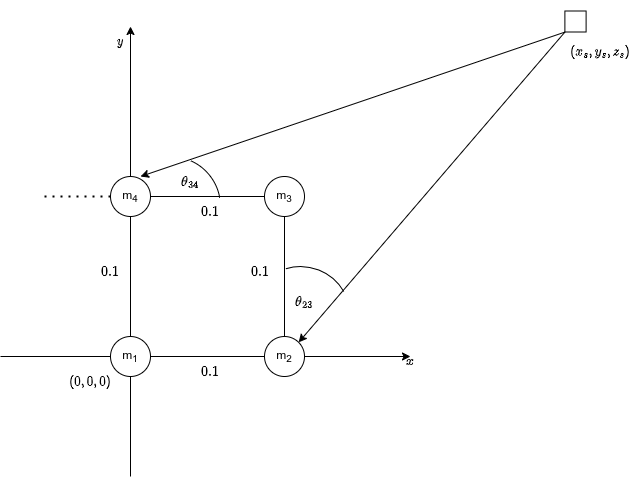
\includegraphics[width=0.68\linewidth]{triangulation_axes.png}
	\caption{Illustrating the angles of arrival for microphone pairs where the angle $\theta_{ij}$, for $i\neq j$, corresponds to the microphone pair $m_i$ and $m_j$.}
	\label{fig:tri_1}
\end{figure}
The simulation created the two microphone arrays using two uniform linear array (ULA) along the $x$-axis of the global coordinate system represented by grid lines on the A1 grid paper. The phase center of the reference microphone pair was assumed to be at ($0$, $0$, $0$) while the second microphone sensor pair was ($0.10$,$0$,$0$) $\si{\meter}$. The direction of the signal from the source located at a point ($x$, $y$ ,$0$) was taken to be in the negative $y$-direction as illustrated in figure\\\\ %\ref{fig:tsource-triangulation-xy-plane}.   
We defined audio signals with different properties and determined the behaviour of the system for different configurations of the microphone array.  The range of frequencies taken into consideration start from 100 Hz and go up to 15 kHz. The simulation assumed a maximum operating range of $\SI{15}{\meter}$ and a speed of sound of $\SI{350}{\meter\per\second}$. We used acoustic chirp signals with noise for analysis since this waveform can be approximated using a Dirac impulse signal. The acoustic chirp was collected by the two pairs of omni-directional microphones spaced at $\SI{0.1}{\meter}$ apart. The azimuth and elevation angles of the acoustic chirp were changed to determine the effectiveness of the configuration design. 

\mysection{5}{Simulation Results \& Discussion}

\subsection{Time Delay Estimation Subsystem Simulation Results}
Microphones were located at shown in the table below, where microphone $m_1$, located at the origin, was used as the reference microphone. The position of the source was changed to determine the accuracy of the time delay algorithm. The example below illustrates the setup of the simulation where the \gls{source} was located at ($1,1,1$) and the microphones were positioned in a square configuration with each side having a length of $\SI{0.1}{\meter}$. This was chosen to satisfy the condition that the distance between microphone pairs cannot be less than half the wavelength of sound waves. 
\begin{figure}[ht!]
	\centering
	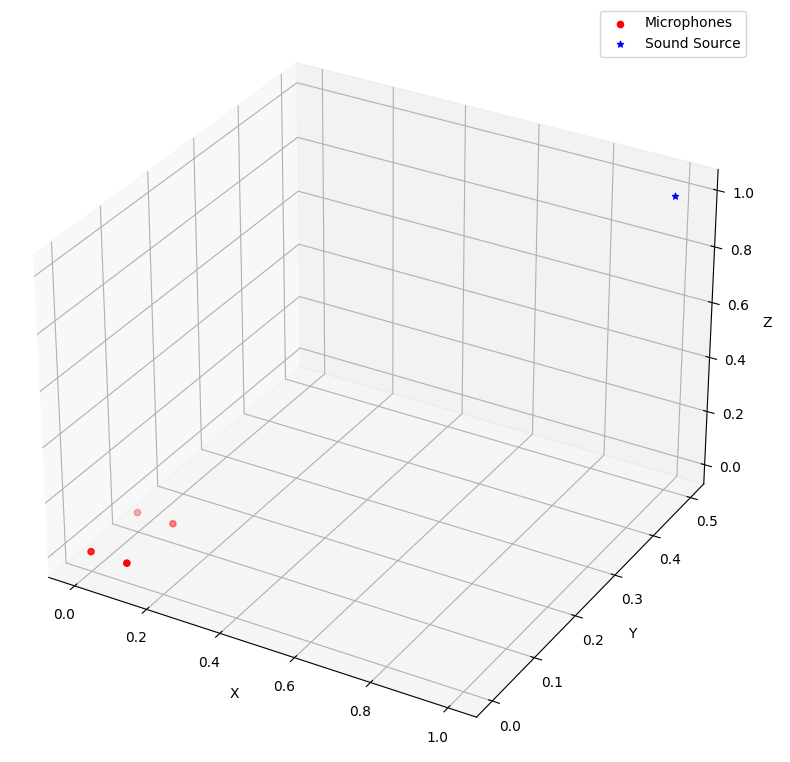
\includegraphics[width=0.8\linewidth]{3d_representation.png}
	\caption{Showing a 3D image of the simulation setup where microphone $m_1$ was located at ($0,0,0$) and the source was located at ($1,1,1$). The microphones were spaced by $\SI{0.1}{\meter}$ apart corresponding to less than half the wave length of sounds in the audible frequency range.}
	\label{fig:microphone_positions}
\end{figure}

The audio signal (\texttt{sound\_signal} variable in \ref{list:signalsim}) was simulated as a mixed sinusoid as illustrated by the code in listing \ref{list:signalsim}. 
\begin{lstlisting}[language=Python, caption={Showing code implementation of an audio signal with mixed freqencies ranging between $\SI{440}{\hertz}$ and $\SI{1760}{\hertz}$.}, label=list:signalsim]
	# Generate a sound signal (sine wave)
	sample_rate = 44100  # Sample rate in Hz
	duration = 0.05  # Duration in seconds
	num_samples = int(duration * sample_rate)
	frequencies = [440.0, 880.0, 1320.0, 1760.0]  # Frequencies in Hz
	t = np.linspace(0, duration, int(sample_rate * duration), endpoint=False)
	
	amplitudes = [0.8, 0.6, 0.4, 0.2]  # Corresponding amplitudes
	
	# Generate the mixed signal
	mixed_signal = np.zeros(num_samples)
	for freq, amp in zip(frequencies, amplitudes):
	mixed_signal += amp * np.sin(2 * np.pi * freq * t)
	# Generate the sound signal (sine wave)
	sound_signal = mixed_signal
\end{lstlisting}
The propagation of sound through air was simulated using the \texttt{simulate\_sound\_propagation} function which had three arguments as shown in \ref{list:soundpropagation}. The default settings of the simulation used a speed of sound of $\SI{346}{\meter\second}$ corresponding to an ambient temperature of $\SI{25}{\degree}$.
\begin{lstlisting}[language=Python, caption={Showing sound propagation simulated given a sinusoidal sound wave, the source position, and microphone positions in 3D.}, label=list:soundpropagation]
	# Sound propagation simulation
	def simulate_sound_propagation(sound_signal, source_position, 
	microphone_position, speed_of_sound, sample_rate):
	# Calculate the distance from the source to the microphone
	distance = np.linalg.norm(source_position - microphone_position)
	# Calculate the time it takes for sound to travel 
	#from the source to the microphone
	travel_time = distance / speed_of_sound
	# Calculate the corresponding sample delay
	sample_delay = int(travel_time * sample_rate)
	
	# Create a delayed version of the sound signal
	delayed_sound_signal = np.zeros_like(sound_signal)
	
	
	if sample_delay < len(sound_signal):
	delayed_sound_signal[sample_delay:] = sound_signal[:-sample_delay]
	
	return delayed_sound_signal
	
	microphone_signals = []
	for mic_position in microphone_positions:
	microphone_signal = simulate_sound_propagation(sound_signal, source_position, mic_position, speed_of_sound, sample_rate)
	microphone_signals.append(microphone_signal)
\end{lstlisting}
The signal at each microphone after implementing the \texttt{simulate\_sound\_propagation} function is shown in figure \ref{fig:signals} for a duration of $\SI{0.5}{\second}$. The figure shows that the signals at each microphone are identical although slightly shifted in time to simulate time delays.
\begin{figure}[ht!]
	\centering
	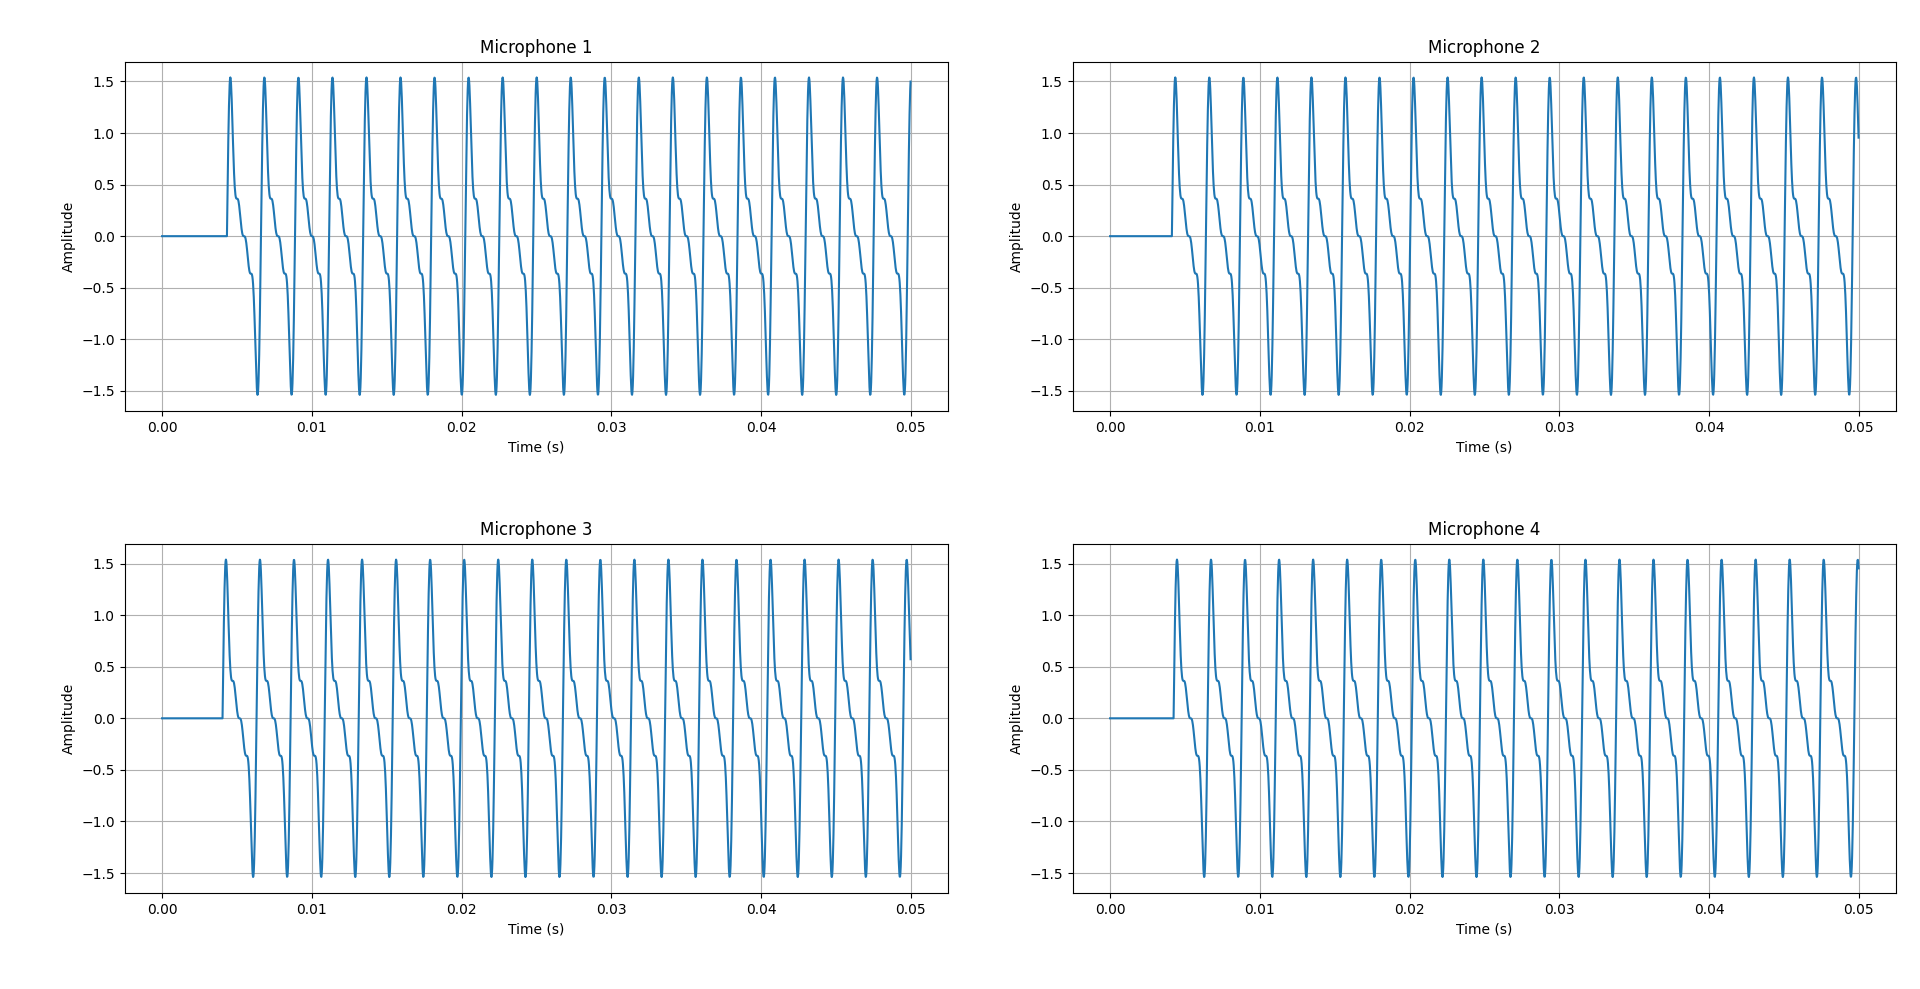
\includegraphics[width=1.1\linewidth]{mic_signals.png}
	\caption{Showing audio signals at each microphone after simulating sound propagation through air using Python.}
	\label{fig:signals}
\end{figure}
Figure \ref{fig:signals_2} shows the signals at the microphones when the source was moved further away to the point ($2,2,2$). A comparison of the figures of the signals for sources located at different points showed accurate time-shift in the signals at the microphones as illustrated by a longer dead-time in the signals where the source was further away compared to a shorter dead-time for a closer source position. This was expected since the speed of sound was taken to be constant, meaning that a sound wave takes longer to reach the microphones when the source is further from the microphones.
\begin{figure}[ht!]
	\centering
	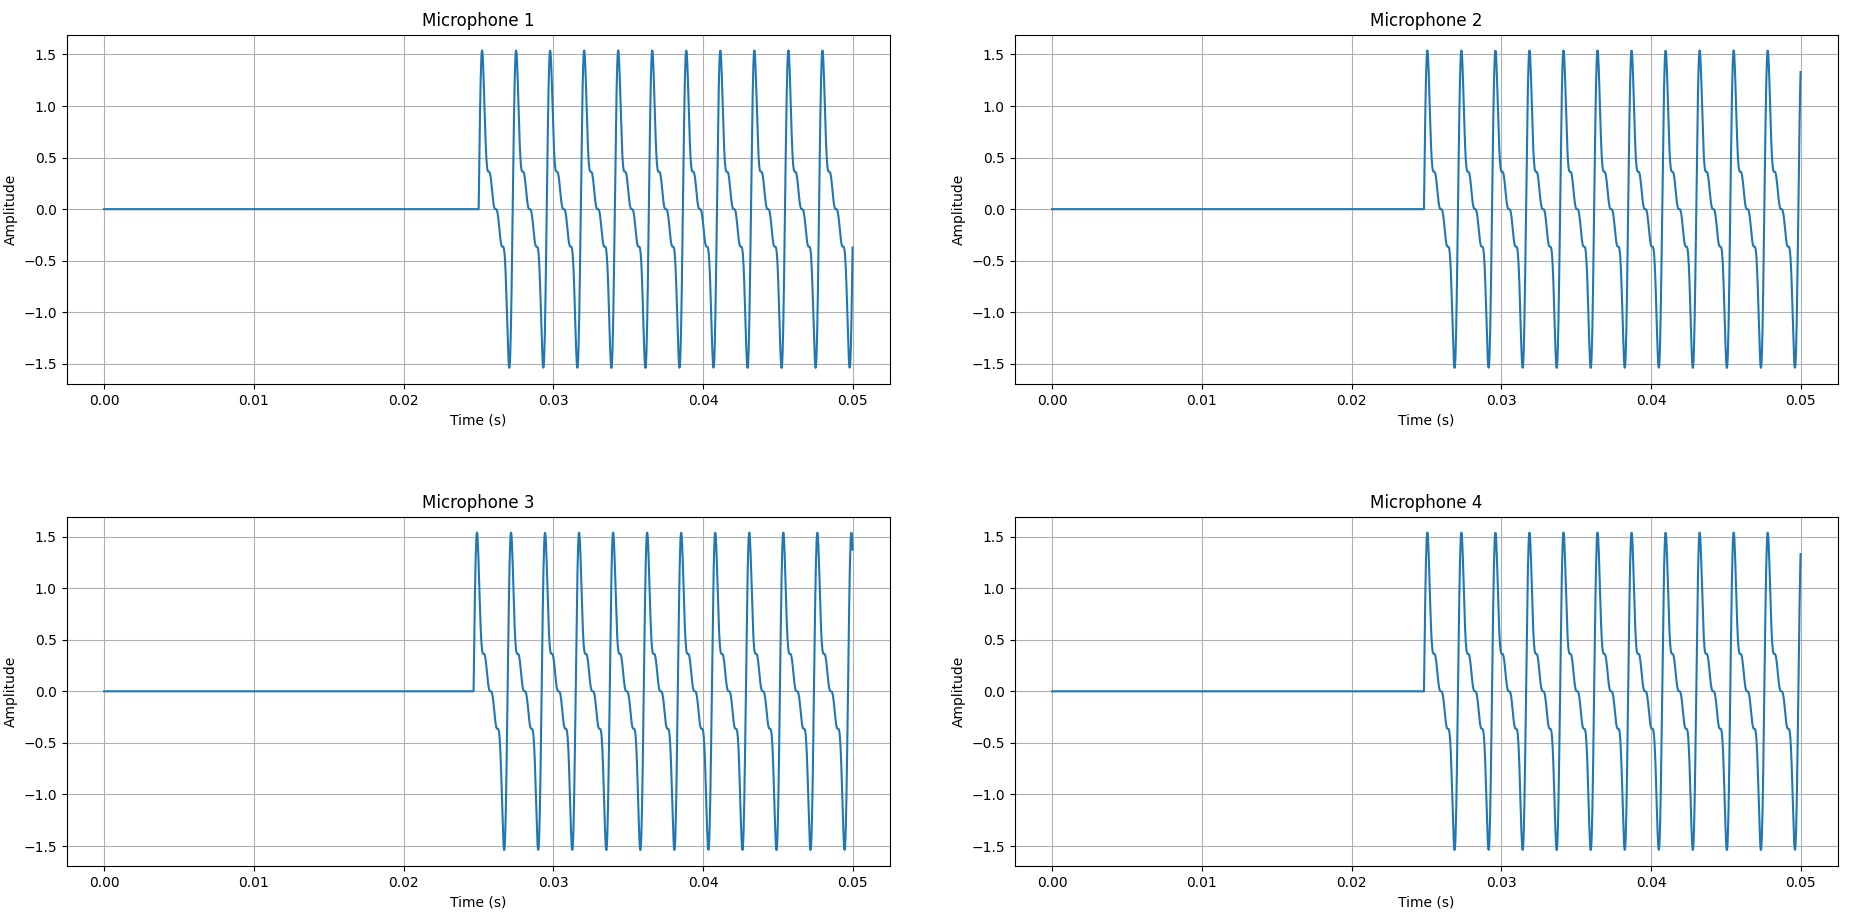
\includegraphics[width=1.1\linewidth]{mic_signals_2.png}
	\caption{Showing a longer dead-time as sound takes longer to travel to microphones compared to the result shown in figure \ref{fig:signals} above.}
	\label{fig:signals_2}
\end{figure}
Time delay estimations were simulated using the code shown in \ref{list:gcc-phat} where the fast Fourier transform function was implemented to find the cross-correlation between the signals at the microphones.
\begin{lstlisting}[language=Python, caption={Showing implementation of GCC-PHAT algorithm to estimate time delays.}, label=list:gcc-phat]
# Compute the GCC-PHAT cross-correlation
def gcc_phat(signal1, signal2):
fft_signal1 = np.fft.fft(signal1)
fft_signal2 = np.fft.fft(signal2)
cross_correlation = fft_signal1 * np.conj(fft_signal2)
cross_correlation /= np.abs(cross_correlation)
inverse_correlation = np.fft.ifft(cross_correlation)
gcc_phat_result = np.abs(inverse_correlation)
return gcc_phat_result
\end{lstlisting}
Results from the implementation of the GCC-PHAT algorithm are illustrated in the figures below. The results show the GCC-PHAT value increased as the source moved away from the reference microphone, and the number of peaks, corresponding to the number of frequencies in the mixed acoustic signal, also increased. This is illustrated by figures \ref{fig:gcc-phat-1} and \ref{fig:gcc-phat-2} showing the GCC-PHAT values obtained when the source was located at points ($1,1,1$), ($2,2,2$), and ($5,5,5$). 
\begin{figure}[ht!]
	\centering
	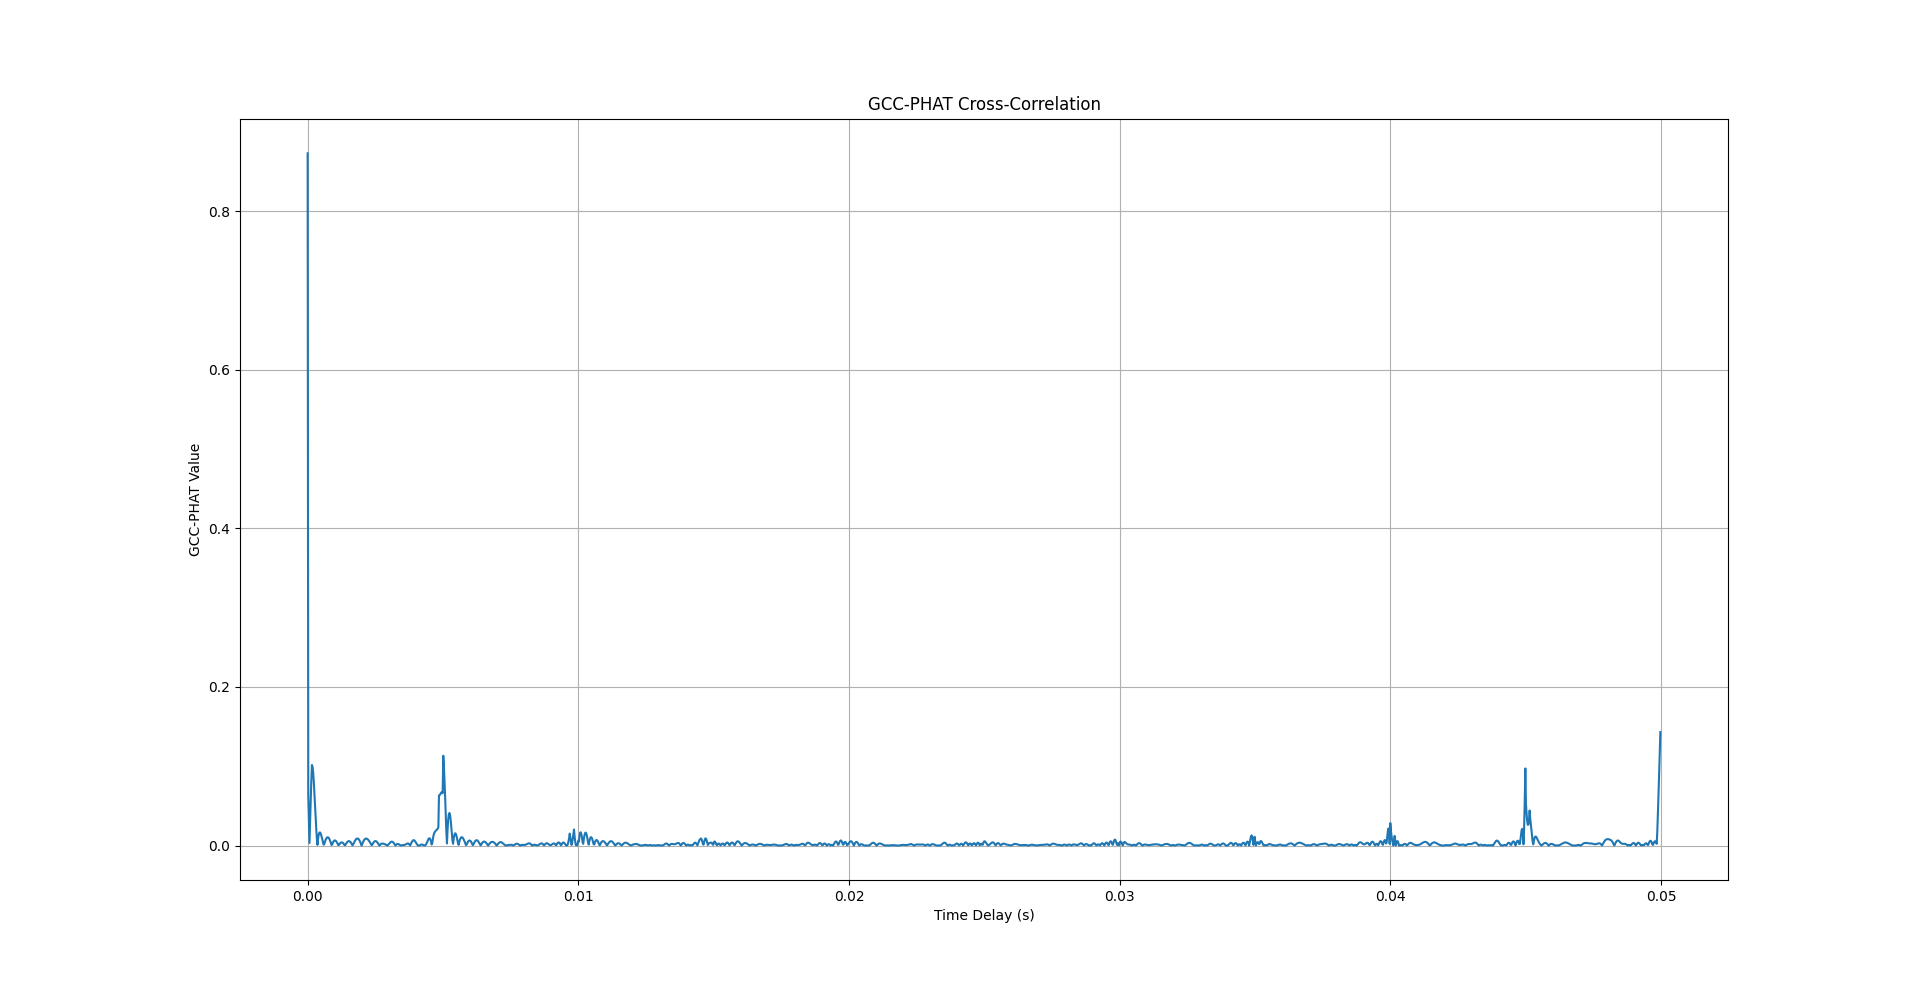
\includegraphics[width=1.0\linewidth]{gcc_phat_1.png}
	\caption{Showing the GCC-PHAT value vs time plot for the cross-correlation analysis between two signals received by microphone pairs when the source was a meter away from the reference microphone.}
	\label{fig:gcc-phat-1}
\end{figure}
\begin{figure}[ht!]
	\centering
	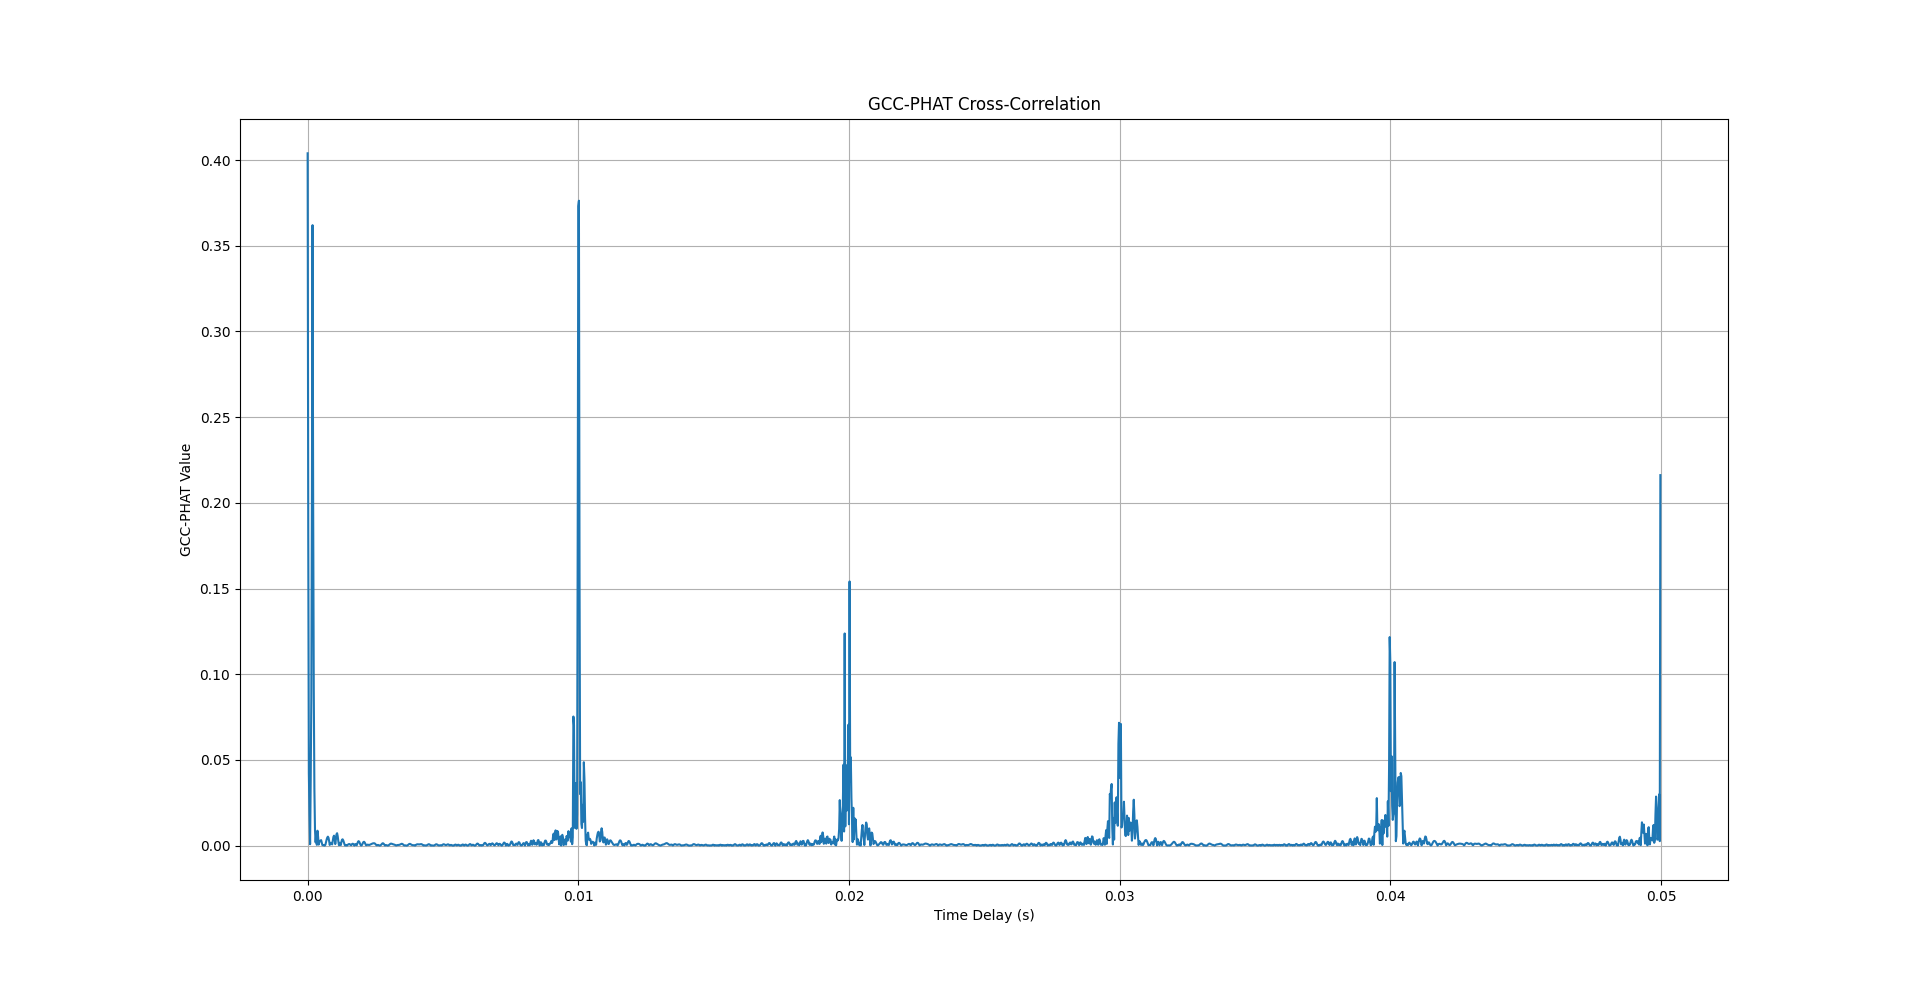
\includegraphics[width=1.0\linewidth]{gcc_phat_2.png}
	\caption{Showing the GCC-PHAT value vs time plot for the cross-correlation analysis between two signals received by microphone pairs when the source was 2 meters away from the reference microphone. More peaks were prevalent as the distance from the origin to the sound source increases.}
	\label{fig:gcc-phat-2}
\end{figure}
\begin{figure}[ht!]
	\centering
	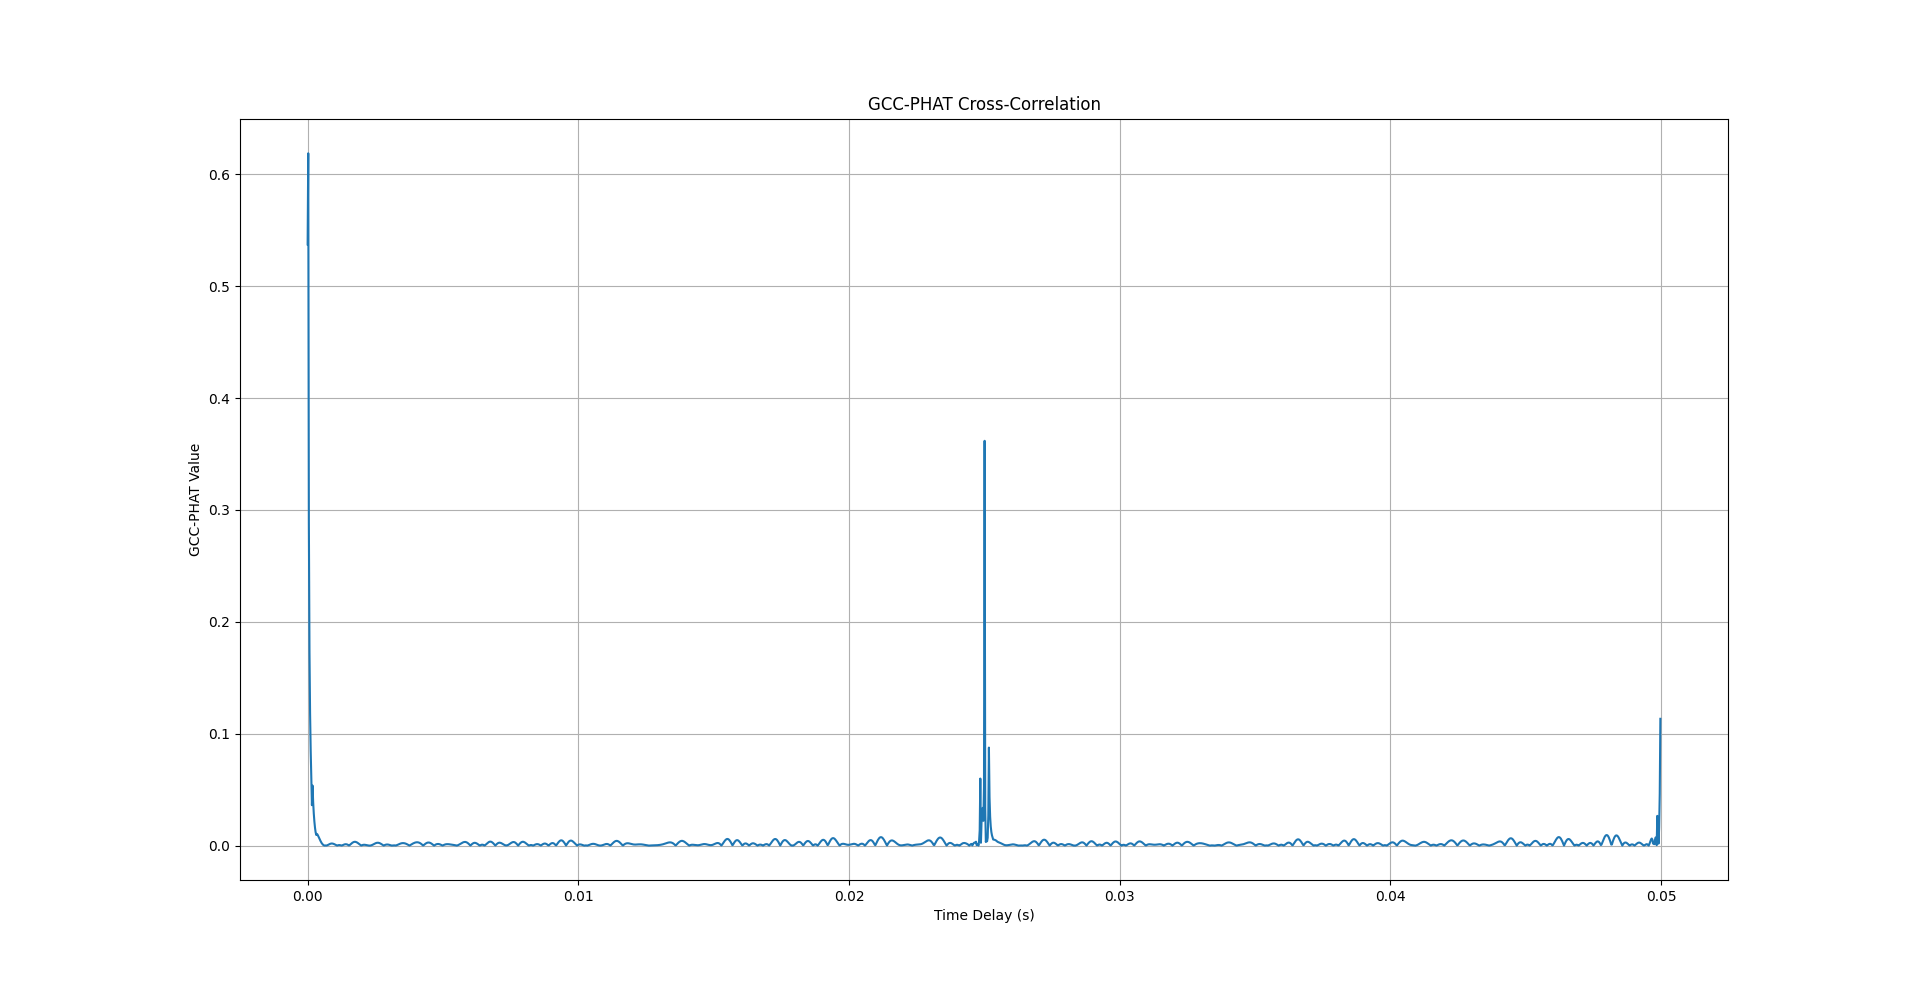
\includegraphics[width=1.0\linewidth]{gcc_phat_5.png}
	\caption{Showing the larger GCC-PHAT value at zero for sound source located further away.}
	\label{fig:gcc-phat-3}
\end{figure}

GCC-PHAT simulations also showed that the correlation between \gls{msigs} signals decreased as the source moved further away from the source as illustrated by the plots below. This result corresponds to the expected behaviour where information about signals is attenuated as it propagates through a medium for a longer distance.
\begin{figure}[ht!]
	\centering
	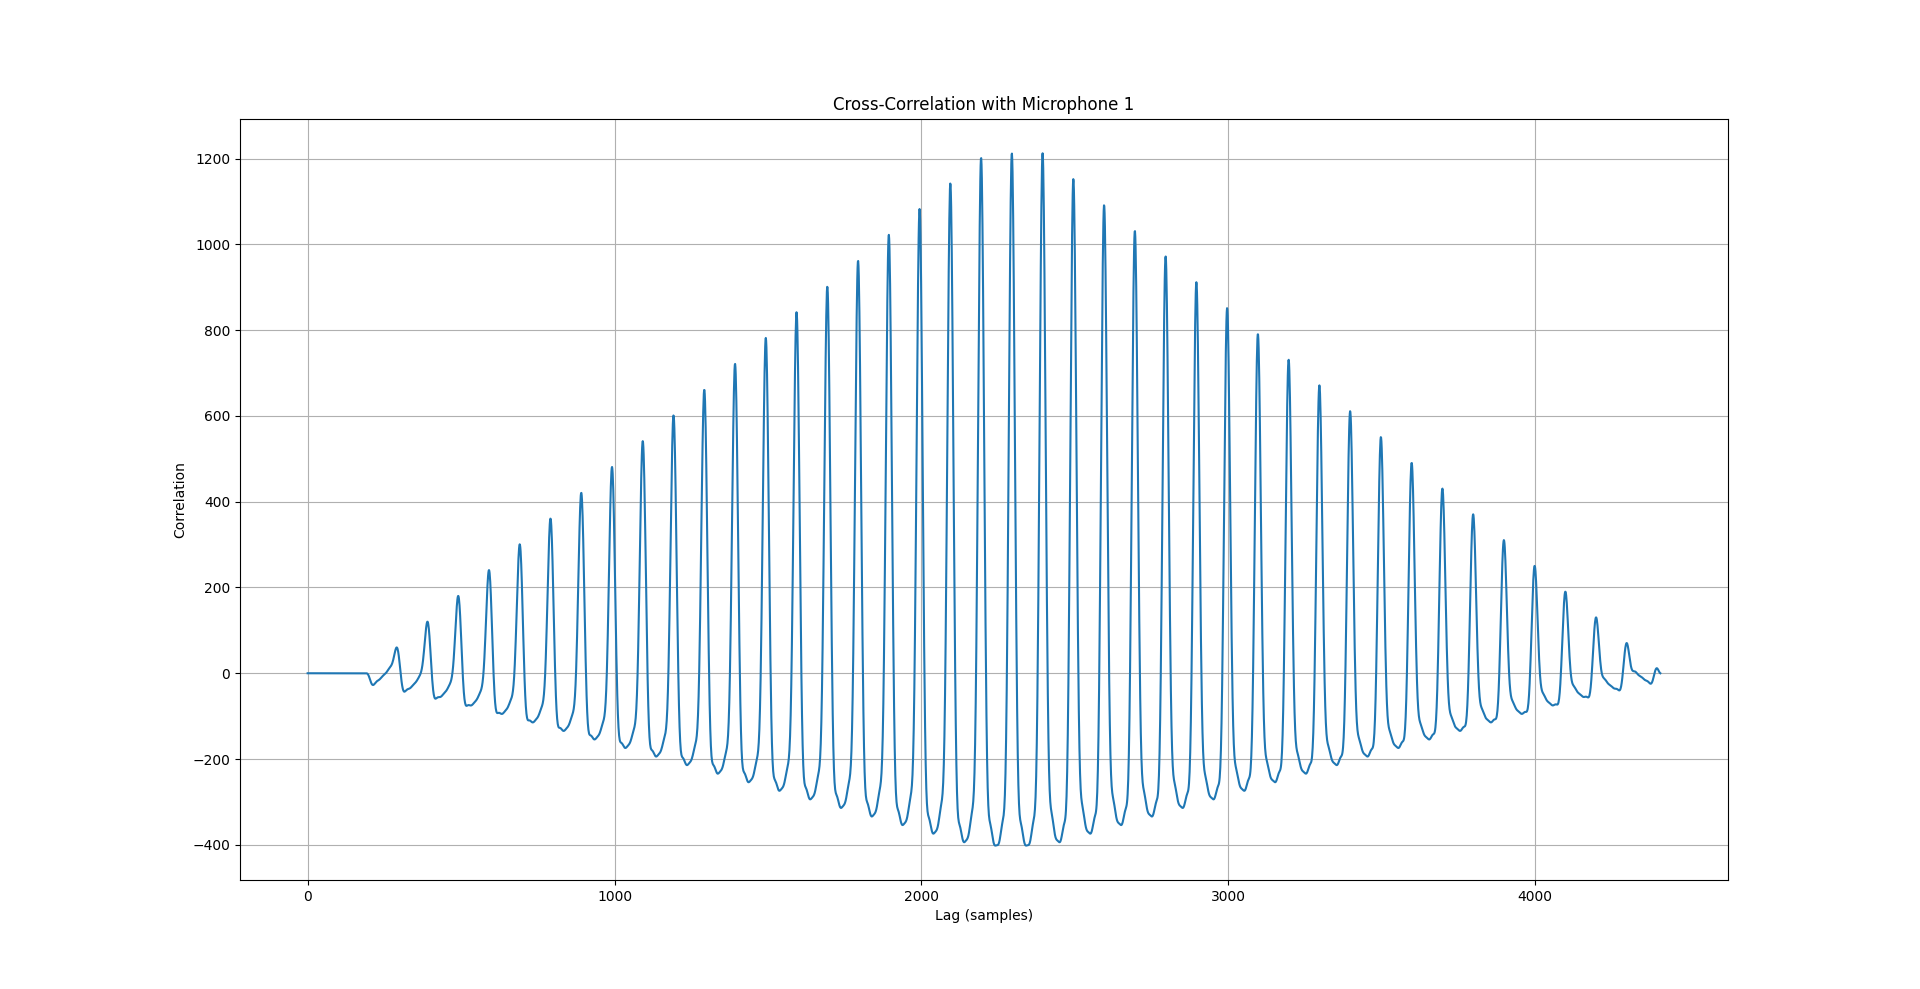
\includegraphics[width=1.0\linewidth]{correlation_1.png}
	\caption{Cross-correlation plot when the source was located at point ($1$,$1$,$1$). The correlation between the signals is highest when the sound emitter is closer to the origin.}
	\label{fig:cross-1}
\end{figure}

\begin{figure}[ht!]
	\centering
	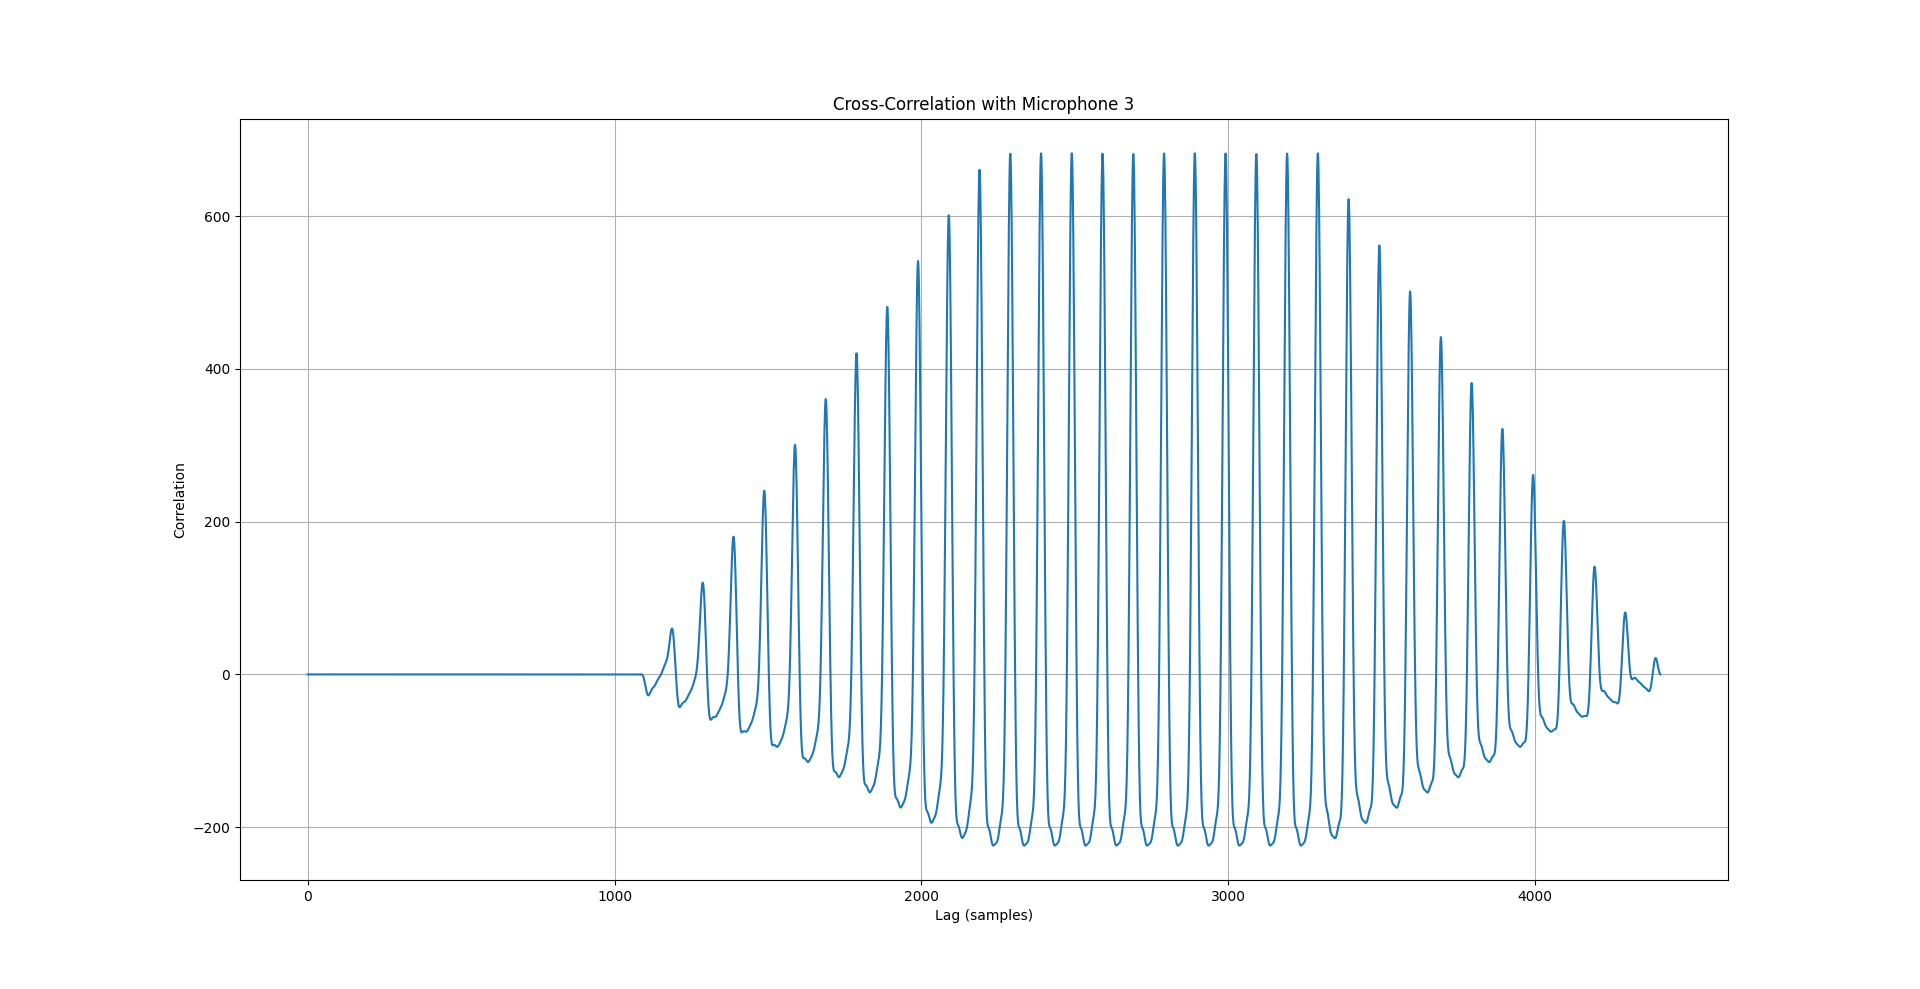
\includegraphics[width=1.0\linewidth]{correlation_5.png}
	\caption{Cross-correlation between microphone signals decreases as the distance to the microphone increases. Here, the sound source was located at point ($5$,$5$,$5$).}
	\label{fig:cross-3}
\end{figure}

\subsection{Triangulation \& Sound-Tracking Subsystem Simulation Results}

Triangulation was simulated using MATLAB where TDoA measurements from a single sound source were used to to localize and track the source in the absence of noise and any other signals that could lead to missed detections. In the triangulation algorithm, time delay estimations were used to determine the direction of arrival of the source as shown in figure \ref{fig:tdoa-diag}. Using the TDoA measurements, the angle of arrival was found to be always adjacent to the longest path taken by sound to reach a microphone pair

\begin{figure}[ht!]
	\centering
	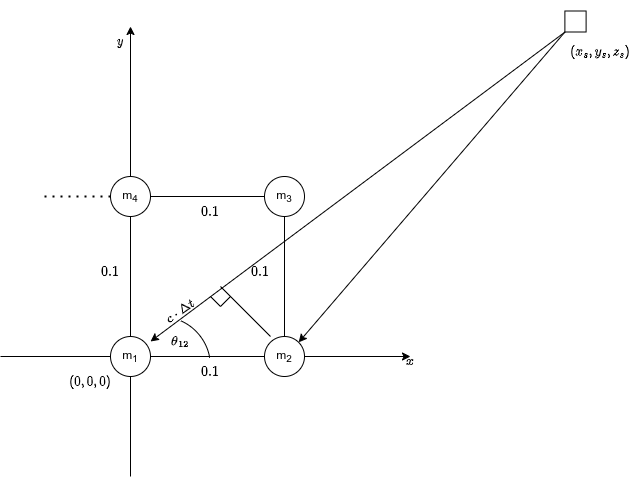
\includegraphics[width=0.8\linewidth]{triangulation_2.png}
	\caption{Angle of arrival used to compute the direction of arrival for microphone pairs.}
	\label{fig:tdoa-diag}
\end{figure}

The MATLAB scrip code snippet shown in listing \ref{list:matlab} tracking shows an implementation of the \texttt{computeSimulateTDOA} function used to simulate the TDoA arrival using the first method described above where the time of arrivals are used to compute the time delay estimations. 

\begin{lstlisting}[language=MATLAB, caption={Showing while loop for continuously tracking the microphone location.}, label=list:matlab]
% Display object
display = ComputeTDOATrackingExampleDisplay(XLimits=[-1e4 1e4],...
YLimits=[-1e4 1e4],...
LogAccuracy=true,...
Title="Single Object Tracking");

% Create a GNN tracker
tracker = trackerGNN(FilterInitializationFcn=@computeInitHighSpeedKF,...
AssignmentThreshold=100);

while advance(scenario)
% Elapsed time
time = scenario.SimulationTime;

% Simulate TDOA detections without false alarms and missed detections
tdoaDets = computeSimulateTDOA(scenario, rxPairs, measNoise);
tdoaseconds = tdoaDets(2)
% Get estimated position and position covariance as objectDetection
% objects
posDet = computeTDOA2Pos(tdoaDets,true);

% Update the tracker with position detections
tracks = tracker(posDet, time);

% Display results
display(scenario, rxPairs, tdoaDets, {posDet}, tracks);
end
\end{lstlisting}
The simulation used the \texttt{computeTDOA2Pos} function to estimate the position and position covariance of the acoustic source at every step using the spherical intersection algorithm. Results were illustrated using an animation as shown in figure \ref{fig:track} where a sound source moves along a track and emits sound towards the microphone array. 

\begin{figure}[ht!]
	\centering
	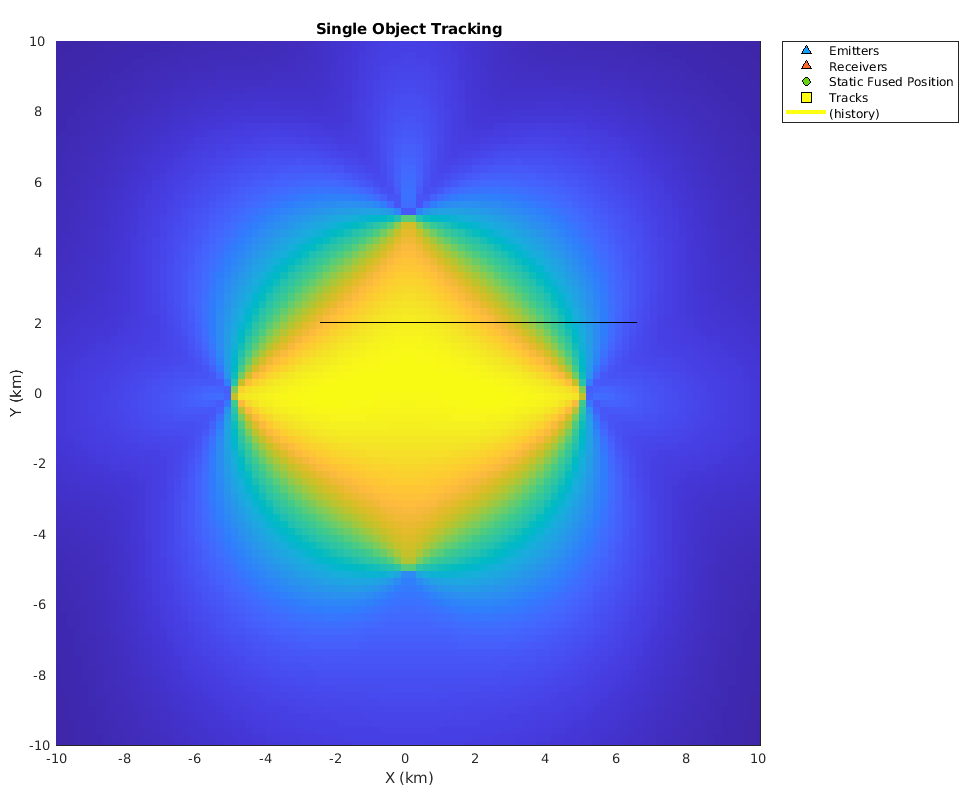
\includegraphics[width=1.0\linewidth]{track.png}
	\caption{Showing sound-tracking simulation in MATLAB where a sound source moves at a constant speed along a straight track.}
	\label{fig:track}
\end{figure}

\mysection{6}{Acceptance Test Procedures}

\subsection{Defining Acceptance Test Procedures}
\textbf{Localization Accuracy:}\\
- Deviation between estimated and actual sound source positions. This will provide insight into the system's precision in determining sound source locations within the grid \\\\
\textbf{Real-time Performance:}\\
- Processing time for sound source localization. This assesses the system's efficiency in processing data in real-time scenarios. \\\\
\textbf{Noise Robustness:}\\
- Ability to accurately localize sound sources in noisy environments. The Signal-to-Noise Ratio (SNR) will be used to quantify the noise level at which accurate localization can still be achieved. \\\\
\textbf{Computational Efficiency:}\\
- Resource utilization and execution time of algorithms. \\\\
\textbf{System Reliability:}\\
- Consistency and stability of results across multiple tests\\\\
\subsection{Outline of Transition to Physical Implementation}
\textbf{1. Hardware Procurement and Setup:} 
\\\\
- Identify and procure the necessary hardware components, including Raspberry Pi Zero boards, MEMS microphones. \\\\
- Determine the physical locations for sensor deployment. \\\\
Install microphones at predefined positions, ensuring the same configuration as in the simulation. 
\\\\
\textbf{2. Software Implementation:}\\
2.1. Porting Simulation Code:\\\\
- Adapt simulation code to work on the Raspberry Pi Zero devices. \\
- Ensure that synchronization mechanisms are effectively implemented.\\\\
2.2. Real-time Processing Optimization: \\\\
- Enhance code for real-time performance. \\
- Optimize algorithms for efficient execution on the hardware. \\\\
2.3. Integration with Hardware: \\\\
- Establish communication protocols between Raspberry Pi Zero devices and microphones. \\\\
- Ensure data acquisition and transmission are functioning correctly. \\\\
\textbf{3. Testing and Calibration:} \\\\
3.1. Hardware Testing: \\\\
- Conduct hardware testing to ensure all components are functioning as expected. \\
3.2. Calibration Procedures: \\\\
- Implement calibration routines for microphone sensitivity and sensor positions.\\\\
\textbf{4. Validation and Performance Testing:} \\\\
4.1. Localization Accuracy Testing: \\\\
- Place sound sources at known positions within the physical environment. \\
- Record and compare estimated positions with actual positions. \\
- Validate the system's accuracy by calculating error metrics. \\\\
4.2. Real-time Performance Assessment: \\\\
- Measure the time it takes for the physical system to calculate sound source positions. \\\\
4.3. Noise Robustness Testing: \\\\
- Introduce controlled levels of background noise. \\
- Evaluate the system's ability to localize sound sources in noisy environments. \\
4.4. Computational Efficiency Analysis: \\\\
- Monitor CPU and memory usage during real-time processing. \\
- Compare execution times with simulation results. \\\\
\textbf{5. Fine-tuning and Optimization:} \\\\
5.1. Algorithm Optimization: \\\\
- Fine-tune algorithms based on physical system performance.\\ 
- Address any discrepancies between simulation and real-world behaviour. \\\\
\textbf{6. Documentation and Reporting:}  \\\\ 
6.1. System Documentation: \\\\
- Document the physical system setup, hardware specifications, and software configurations. \\\\
6.2. Performance Report: \\\\
- Generate a comprehensive report detailing the physical system's performance. \\
- Include results of accuracy, real-time performance, noise robustness, and efficiency tests. \\\\
\textbf{7. Deployment and Integration:} \\\\
7.1. Integration with Application: \\\\
- Integrate the sound source localization system with the intended platform. 

\mysection{7}{Conclusion}

In this study, we conducted simulations to assess the performance of the Time Delay Estimation and Triangulation subsystems for sound source localization in a 3D space. The following key findings and conclusions can be drawn from our simulations:

\subsection{Time Delay Estimation Subsystem}

1. The Time Delay Estimation Subsystem demonstrated accurate estimation of time delays between microphone pairs, even for complex mixed-frequency sound signals. The GCC-PHAT algorithm successfully identified time delays, which increased as the source moved further away from the reference microphone.

2. The correlation between microphone signals decreased as the source moved farther from the reference microphone, reflecting the expected attenuation of signals over longer distances.

3. Simulation results validated the capability of the subsystem to provide precise time delay estimations, crucial for accurate sound source localization.

\subsection{Triangulation \& Sound-Tracking Subsystem}

1. Triangulation simulations successfully localized sound sources in 3D space using Time Difference of Arrival (TDoA) measurements. The direction of arrival was computed using the angle adjacent to the longest sound path between microphone pairs.

2. The subsystem demonstrated its ability to accurately track sound sources' movements in a noise-free environment, making it suitable for applications requiring real-time sound tracking.

In conclusion, the simulations showcased the effectiveness and accuracy of the Time Delay Estimation and Triangulation subsystems for sound source localization and tracking in 3D space. Future work may involve incorporating noise models and real-world conditions to further validate the subsystems' performance in practical applications.

\addcontentsline{toc}{section}{References}
\bibliographystyle{ieeetr}
\bibliography{references}

\clearpage

\addcontentsline{toc}{section}{Appendices}
\subsection*{Appendix A: Link To Acoustic-Triangulation-Github Link}

\url{https://github.com/BongaNjamela001/Acoustic-Triangulation-System}

\end{document}